%%notwendige packages

%----------------------------

\documentclass[12pt, twoside]{article}
%benötigt man immer
\usepackage{amsmath}
%is used for numbering of equations
\usepackage[english]{babel}
\usepackage[utf8x]{inputenc}
\usepackage{varwidth}
\usepackage{float}
% Table caption on top of tables
%\floatstyle{plaintop}
\restylefloat{table}
%----
\usepackage{makecell}
\usepackage{enumitem}

% Für fette Mathesymbole
\usepackage{amsfonts}
\usepackage{amsthm}
\usepackage{bm}
\renewcommand*{\mathbf}[1]{\ifmmode\bm{#1}\else\textbf{#1}\fi}
\usepackage{physics}


% Don't use natbib, it messes up everything with fancyhdr for headnotes.
% You can load this AFTER fancyhdr I gues...
%\usepackage[square]{natbib}



% Create links to references etc.. Usually with function autoref{}...
\usepackage{hyperref}


% For the type of citation and bibliographic style
%\usepackage{apacite}

% allows index generation
\usepackage{makeidx}
\makeindex

% equation, table and figure numbering should start with section number e.g. (3.1)
\numberwithin{equation}{section}
\numberwithin{table}{section}
\numberwithin{figure}{section}

%fonts
\usepackage[T1]{fontenc}

\usepackage{uarial}
\renewcommand{\familydefault}{\sfdefault}
\usepackage{blindtext}

\usepackage{textcomp}
%\usepackage{mathptmx}
\usepackage{tabularx}
\usepackage{multirow}
\usepackage{enumitem}
%small fonts for captions of figures and tables
\usepackage[center]{caption}
\captionsetup[figure]{font = footnotesize}
\captionsetup[table]{font = footnotesize}


%format
% Witwen und Waisenkinder vermeiden
\clubpenalty=4500	% Waisen vermeiden (erste Zeile eines neuen Absatzes als letzte Zeile einer Seite)
\widowpenalty=10000	% keine Witwen zulassen (letzte Zeile eines Absatzes am Beginn einer neuen Seite)

% Seitenraender einstellen
\usepackage{geometry}
\geometry{a4paper,left=30mm,right=30mm, top=20mm, bottom=20mm}

% Zeilenabstand
\linespread{1.5} 

% Disable indentation for the entire document
\setlength\parindent{0pt}

% turn off hyphenation and justification (Silbentrennung ausschalten)
\tolerance=1
\emergencystretch=\maxdimen
\hyphenpenalty=10000
\hbadness=10000

%Graphics
\usepackage[final]{graphicx} 	
\usepackage[twoside,figuresright]{rotating}
\usepackage{subcaption} 
%\usepackage{subfigure} 

% Adjust tables (and figures) to textwidth...
\usepackage{adjustbox}

%For tables, to color whole row without missing pieces...
\usepackage{tabularx}
%\usepackage[table]{xcolor}  % option loads »colortbl«

% Initialize Makro for table heads
\renewcommand\theadfont{\bfseries\sffamily}

% Highlighting rows, columns and headers of tables
\usepackage{color, colortbl}
\definecolor{Gray}{gray}{0.9}
\definecolor{LightCyan}{rgb}{0.88,1,1}
\definecolor{SeaBlue}{rgb}{0.3, 0.58, 1}

%acronym package for Abbreviations
\usepackage{acronym}
% macro for first letter capital (e.g. in new sentence)
%\usepackage{etoolbox}


%package to capitalize first letter in a word. Use function 
%\capitalisewords{first letter upper case}
%\usepackage{mfirstuc}

%Create Statutory Declaration page for signatures
\newcommand{\namesigdate}[2][3cm]{%
  \begin{tabular}{@{}p{#1}@{}}
    #2 \\[2\normalbaselineskip] \hrule \\[0pt]
    {\small \textit{Signature}}
  \end{tabular}
}

% Headers for the pages
%\usepackage{fancyhdr}
%\pagestyle{headings}

%\fancyhf{}

\usepackage{fancyhdr}
\pagestyle{fancy}
% Clear page setup with \fancyhf{}
\fancyhf{}
% The next two lines we dont need yet..
%\fancyhead[LO,RE]{\footnotesize \nouppercase{\leftmark}}
%\fancyhead[RO,LE]{\footnotesize \thepage}
%\fancyfoot[C]{\thepage}
\renewcommand{\headrulewidth}{1pt}
% Hide section number in headnote
%\renewcommand\sectionmark[1]{\markboth{#1}{}}


% For individual page numbering, change the 
% "plain" command in \thispagestyle
\makeatletter
\def\ps@plain{\let\@mkboth\@gobbletwo
  \let\@oddhead\@empty
  \def\@oddfoot{\reset@font\hfill\thepage}% page number on right
  \let\@evenhead\@empty
  \let\@evenfoot\@oddfoot}
\makeatother

% This line has to come AFTER package fancyhdr and pagestyle fancy
\usepackage[square]{natbib}


%----------------------------

\begin{document}

\thispagestyle{empty}	
% !TEX root = Master.tex

%titlepage
\thispagestyle{empty}
\begin{center}


\begin{minipage}{0.75\linewidth}
    \centering
%University logo
    
\includegraphics[scale = 0.7]{figures/uni_goettingen_logo.pdf}\\
    
    %\rule{0.4\linewidth}{0.15\linewidth}\par
    \vspace{1cm}
    
% Master Thesis
{{\Huge \textbf{Master Thesis} \par}}
    
\vspace{0.5cm}
    
%Thesis title
    {{\LARGE Multivariate modelling of the dependency structure between article sales of a sportswear manufacturer\par}}
    \vspace{1cm}
    
    
%Author's name
\begin{center}
Author\\
{\LARGE \textbf{Petros Christanas}} \\
{\large from Nuremberg}


\vspace{0.5cm}

Matriculation Number \\
{\large 11604278}

\vspace{1cm}

{\Large Applied Statistics M.Sc.}\\
{\large Chair of Statistics and Econometrics}

\end{center}
    
    \end{minipage}
\end{center}


\vspace{1.5cm}

\noindent Supervisors\\
\noindent {\Large \textbf{Prof. Dr. Thomas Kneib}} \\
\noindent {\Large \textbf{Dipl.-Vw. Quant. Fabian H. C. Raters}} \\

\vspace{0.5cm}
    
%Date
\begin{flushleft}
\noindent {\normalsize Submitted \today} \\
\noindent {\normalsize Processing time of 20 weeks}
\end{flushleft}

    
    

\clearpage

%One empty page. Left pages empty before contents..
\newpage
\null\thispagestyle{empty}
\newpage


\thispagestyle{empty}
\section*{Confidentiality Clause}
%\input{confidentiality_clause}
\clearpage

%Empty page 
\newpage
\null\thispagestyle{empty}

\newpage
\thispagestyle{empty}
\section*{Statutory Declaration}
%\input{statutory_declaration}
\clearpage

\newpage
\null\thispagestyle{empty}


\newpage
\thispagestyle{empty}
\section*{Acknowledgments}
%\input{acknowledgments}
\newpage
\null\thispagestyle{empty}
\newpage


	
\fancyhf{}
\fancyhead[LO,RE]{\footnotesize \nouppercase{\leftmark}}
% But we don't want the page in contents, so we comment out netxt line
%\fancyhead[RO,LE]{\footnotesize \thepage}
\thispagestyle{empty}
\tableofcontents
%\addtocontents{toc}{\protect\thispagestyle{empty}}
%\pagenumbering{gobble}
\newpage


% Now clear headnotes again and get settings
\fancyhf{}
\fancyhead[LO,RE]{\footnotesize \nouppercase{\leftmark}}
\fancyhead[RO,LE]{\footnotesize \thepage}



\pagenumbering{arabic} 
\setcounter{page}{1} 



\thispagestyle{plain}
\section{Introduction} \label{sec:introduction}
\input{introduction}
\subsection{adidas} \label{ssec:adidas}
%% !TEX root = Master.tex


The \textit{"Dassler Brothers Shoe Factory"} (German: \textit{"Gebrüder Dassler Schuhfabrik"}), which was led by \textit{Adolf Dassler} (aka \textit{Adi Dassler}) and his brother Rudolph, was dissolved in 1947. The brothers split up and formed their own firms. As a result, the sports shoe factory \textit{"Adi Dassler adidas Sportschuhfabrik"} was founded on August 18th 1949 by Adolf Dassler in Herzogenaurach, a small town in Germany \citep{adidas-group}. \\

\begin{figure}[H]
\centering
\begin{subfigure}{.4\textwidth}
  \centering
  \includegraphics[width=\linewidth]{figures/adidas_performance_logo.eps}
  \caption{adidas Performance}
  \label{fig:adidas_performance_logo}
\end{subfigure}
\begin{subfigure}{.4\textwidth}
  \centering
  \includegraphics[width=\linewidth]{figures/adidas_originals_logo.eps}
  \caption{adidas Originals}
  \label{fig:adidas_originals_logo}
\end{subfigure}
\caption{Two of the adidas-group logos: Performance (left) \& Originals (right) \\ \citep{adidasmediacenter}}
\label{fig:adidas_logos}
\end{figure} 


Today, just over 70 years later, the sportswear designer and manufacturer is known as the \textit{"adidas AG"} (short: \textit{adidas}) and is one of the world's biggest sports and fashion brands. The global headquarters of are located in the birthplace Herzogenaurach and the company is employing over 59,000 people worldwide, with \textit{Kasper R\o rsted} leading the brand as CEO since October 1st 2016. In 2019, adidas produced over 1.1 billion sports and sports lifestyle products \citep{adidas-group-profile} and is nowadays sponsoring a vast range of athletes, artists and organizations across the globe (e.g. the  \href{https://www.fifa.com/worldcup/}{FIFA World Cup\texttrademark}).\\

\begin{figure}[H]
\centering
  
\includegraphics[width=.95\linewidth]{figures/adidas_70_years.eps}
  \caption{adidas celebrates its 70th anniversary and the opening of the ARENA building \citep{adidas70years}}
  \label{fig:adidas_70_years}
\end{figure}

With the company's rapid growth, the data produced and acquired from social media, e-Commerce (eCom), transactions, demographics and other channels require suitable instruments and stuff to generate business relevant insights. As the need for data-driven decision making keeps increasing, \textit{"Data and Analytics (DNA)"} became a sub-department of IT. Within DNA, the \textit{"Data Science \& AI Solutions"} team consisting of data scientists, analysts, engineers and other roles is responsible for carrying out analytical tasks, for the most part in the context of numerous DNA use cases.










\subsection{Data Sources} \label{ssec:data_sources}
% !TEX root = Master.tex

Throughout each season, transactional data are collected from online purchases of the sports brand's eCommerce website. Specifically, we are provided with weekly sales data for western European countries depicted in table \ref{tab:transactional_data}.

\begin{table}[H]
\setlength\arrayrulewidth{1pt}  
\centering
\begin{adjustbox}{max width=\textwidth}
\begin{tabular}{|l|l|l|}
\hline
\rowcolor{Gray} 
\textbf{Column}         & \textbf{Description}                                                                                                        & \textbf{Values}              \\ \hline
week\_id                & Calender week of a specific year (YYYYWW)                                                                         & Factors:\textit{ 201648, ..., 201852}          \\ \hline
article\_number         & Unique article identification number (article ID)                                                                           & Factors: \textit{10669, 10, ...       }        \\ \hline
min\_date\_of\_week     & \begin{tabular}[c]{@{}l@{}} Minimum date of the respective week; always a Monday \\ (YYYY-MM-DD)                                                          \end{tabular} & Dates: \textit{2016-11-28, ..., 2018-12-24}  \\ \hline
art\_min\_price         & Minimal recorded price of the article                                                                                       & Non-negative (integer) value \\ \hline
month\_id               & Calender month of a specific year (YYYYMM)                                                                               & Factors: \textit{201612, ..., 201812}          \\ \hline
season                  & \begin{tabular}[c]{@{}l@{}}Season of year (format: SSYY) \\ (Spring-Summer [SS]:  December - May)\\  Fall-Winter [FW]: June - November)\end{tabular} & \begin{tabular}[c]{@{}l@{}}  Factors: \\ \textit{SS17, FW17,} \\\textit{ SS18, FW18, SS19} \end{tabular} \\

 \hline
bf\_w                   & Weekly "Black Friday" promotion intensity of the article                                                                    & Between 0 and 1              \\ \hline
ff\_w                   & Weekly "Friends \& Family" promotion intensity of the article                                                               & Between 0 and 1              \\ \hline
ot\_w                   & Weekly article promotion intensity of "Other" type                                                                          & Between 0 and 1              \\ \hline
gross\_demand\_quantity & Weekly amount of added articles to shopping cart                                                                            & Non-negative (integer) value \\ \hline
base\_price\_locf       & Retail price of the article without any discounts                                                                           & Non-negative (integer) value \\ \hline
total\_markdown\_pct    &                                                                                                                             &                              \\ \hline
day\_of\_month          & Day of the month                                                                                                            & Integers: \textit{1 - 31}                       \\ \hline
month\_of\_year         & Month of the year                                                                                                           & Factors: \textit{January, ..., December}       \\ \hline
year                    & Year                                                                                                                        & Integers: \textit{2016, 2017, 2018}             \\ \hline
week\_of\_year          & Week of the year                                                                                                            & Integers: \textit{1 - 52}                       \\ \hline
\end{tabular}
\end{adjustbox}
\caption{Transactional raw data description from online purchases of western European countries}
\label{tab:transactional_data}
\end{table}

Due to legal regulations of the company, some columns had to undergo anonymization in order for the data to be released. To ensure data protection and confidentiality, numeric variables (with exception of time-indicating columns) were transformed. As a consequence for the analysis part, most integer values were converted to float numbers. This fact should be kept in mind by the reader, since the above table serves as a reminder and reference point for the data documentation.\\

Another peculiarity of this setup is to be considered, too. We will often refer to the variable \textit{gross demand quantity} as \textit{sales}, even though it is obviously not exactly the same. In the eCommerce environment, there are several stages before the purchase is complete, e.g. addition to cart, removal from cart, proceeding to checkout \& even the return of bought articles. Targeting the articles added to cart, i.e. the (gross) demand quantity, provides the optimal data extraction for analytical purposes and is the closest to adequately model the dependency structure between net sales of articles.\\

Besides the transactional data, \textit{article master data}, i.e. attributes of the articles, are provided and depicted in table \ref{tab:article_master_data}.

\begin{table}[H]
\setlength\arrayrulewidth{1pt}  
\centering
\begin{adjustbox}{max width=\textwidth}
\begin{tabular}{|l|l|l|}
\hline
\rowcolor{Gray} 
\textbf{Column}         & \textbf{Description}                                                                                                        & \textbf{Values}              \\ \hline
week\_id                & Calender week of a specific year (YYYYWW)                                                                         & Factors:\textit{ 201648, ..., 201852}          \\ \hline
article\_number         & Unique article identification number (article ID)                                                                           & Factors: \textit{10669, 10, ...       }        \\ \hline
min\_date\_of\_week     & \begin{tabular}[c]{@{}l@{}} Minimum date of the respective week; always a Monday \\ (YYYY-MM-DD)                                                          \end{tabular} & Dates: \textit{2016-11-28, ..., 2018-12-24}  \\ \hline
art\_min\_price         & Minimal recorded price of the article                                                                                       & Non-negative (integer) value \\ \hline
month\_id               & Calender month of a specific year (YYYYMM)                                                                               & Factors: \textit{201612, ..., 201812}          \\ \hline
season                  & \begin{tabular}[c]{@{}l@{}}Season of year (format: SSYY) \\ (Spring-Summer [SS]:  December - May)\\  Fall-Winter [FW]: June - November)\end{tabular} & \begin{tabular}[c]{@{}l@{}}  Factors: \\ \textit{SS17, FW17,} \\\textit{ SS18, FW18, SS19} \end{tabular} \\

 \hline
bf\_w                   & Weekly "Black Friday" promotion intensity of the article                                                                    & Between 0 and 1              \\ \hline
ff\_w                   & Weekly "Friends \& Family" promotion intensity of the article                                                               & Between 0 and 1              \\ \hline
ot\_w                   & Weekly article promotion intensity of "Other" type                                                                          & Between 0 and 1              \\ \hline
gross\_demand\_quantity & Weekly amount of added articles to shopping cart                                                                            & Non-negative (integer) value \\ \hline
base\_price\_locf       & Retail price of the article without any discounts                                                                           & Non-negative (integer) value \\ \hline
total\_markdown\_pct    &                                                                                                                             &                              \\ \hline
day\_of\_month          & Day of the month                                                                                                            & Integers: \textit{1 - 31}                       \\ \hline
month\_of\_year         & Month of the year                                                                                                           & Factors: \textit{January, ..., December}       \\ \hline
year                    & Year                                                                                                                        & Integers: \textit{2016, 2017, 2018}             \\ \hline
week\_of\_year          & Week of the year                                                                                                            & Integers: \textit{1 - 52}                       \\ \hline
\end{tabular}
\end{adjustbox}
\caption{Article master data}
\label{tab:article_master_data}
\end{table}




\subsection{Motivation} \label{ssec:motivation}
%% !TEX root = Master.tex

What is the motivation and purpose of this thesis...\\
Write also towards the end..
\newpage
\thispagestyle{empty}
\cleardoublepage

\thispagestyle{plain}
\section{Statistical Theory \& Methods} \label{sec:theory_and_methods}
% !TEX root = Master.tex

This chapter introduces various statistical methods used during the conduction of this thesis. Basic notations regarding mathematical foundations of statistics (such as linear algebra, probability theory, etc) are skipped. The chapter starts off with some fundamental notions on generalized linear models and arrives at a brief introduction to additive models


\subsection{Generalized Linear Models} \label{ssec:glm}
% !TEX root = Master.tex
\textit{\acp{GLM}} are an extension of the classical \textit{\ac{LM}}
\begin{equation}
\begin{aligned}
&y_{i}=\beta_{0}+\beta_{1} x_{i 1}+\ldots+\beta_{k} x_{i k}+\varepsilon_{i}, &i=1, \ldots, n
\end{aligned}
\end{equation}
which in matrix notation can be written as
\begin{equation}
 \bm{y} = \bm{X}\bm{\beta} + \bm{\varepsilon} 
\end{equation}
where the response variable $y_i$ can take values from several probability distributions (e.g. Poisson, Binomial, Gamma, ...), which are members of the exponential family \citep{fahrmeir2003regression}. The linear predictor 
\begin{equation} 
\eta_i = \beta_{0}+\beta_{1} x_{i 1}+\ldots+\beta_{k} x_{i k}+\varepsilon_{i} = \bm{x'}_i \bm{\beta} + \bm{\varepsilon}
\label{eq:linear_predictor_glm}
\end{equation}
is passed through a \textit{response function h} (a one-to-one, twice differentiable transformation), such that
\begin{equation}
 E(y_i) = h(\eta_i),
\label{eq:response_function}
\end{equation}
where $h$ ensures that the expected value of the response variable belongs to the appropriate value range. The inverse of the response function, i.e.
\begin{equation}
g = h^{-1},
\label{eq:link_function}
\end{equation} 
is called the \textit{link function} and transforms the mean of the response's distribution to an unbounded continuous scale.

% MAXIMUM LIKELIHOOD ESTIMATION HERE??...




\subsection{Mixed Effects Models} \label{ssec:mixed_models}
% !TEX root = Master.tex
\textit{\acp{LMM}} are powerful tools when dealing with clustered data or data with a longitudinal structure (repeated measurements of individuals).
As in the classical \ac{LM}, there are population-specific effects, namely the parameter vector of \textit{fixed effects} $\boldsymbol{\beta}$, as well as the cluster- or individual-specific effects of such models called \textit{random effects} \citep{fahrmeir2003regression}. 
%In the following, we will refer to our clusters or
%individuals as \textit{"groups"} for briefness.
Mathematically speaking, the linear predictor $\eta_{ij}= \mathbf{x}'_{ij} \mathbf{\beta} $ is extended to
\begin{equation}
\eta_{ij} = \bm{{x'}}_{ij} \bm{\beta} + \bm{u'}_{ij}\bm{\gamma}_i  
\label{eq:linear_mixed_predictor}
\end{equation}
for individuals $i=1, \ldots, m$ measured in a longitudinal setting at observed times $t_{i1} < \ldots < t_{ij} < \ldots < t_{i_{n_i}}$
or for subjects $j=1, \ldots, n_i$ in cluster $i=1, \ldots, m$. \\
In any case,
\begin{itemize}
\item $\bm{\beta}$ is the vector of fixed effects,
\item $\bm{\gamma}_i$ is the vector of random effects,
\item $\bm{x'}_{ij}$ is the vector of covariates and
\item $\bm{u'}_{ij}$ is a subvector of $\bm{x'}_{ij}$.
\end{itemize}


$\bm{x'}_{ij} = (1, x_{ij1}, \ldots, x_{ijk}) $ and $ \bm{u'}_{ij} = (1, u_{ij1}, \ldots, u_{ijk}) $ are therefore the design vectors and $\varepsilon_{ij}$ are the error terms of the \textit{measurement model}\footnote{More details on the vector and matrix forms can be found in the appendix.} specified as

\begin{equation}
y_{ij} =  \bm{x'}_{ij} \bm{\beta} + \bm{u'}_{ij} \bm{\gamma}_i + \varepsilon_{ij}, \quad \varepsilon_{i j} \overset{i.i.d.} \sim N\left(0, \sigma^{2}\right) 
\end{equation}
or in matrix notation

\begin{equation}
\bm{y}_{i}=\bm{X}_{i} \bm{\beta} + \bm{U}_{i} \bm{\gamma}_{i} + \bm{\varepsilon}_{i}
\end{equation}
with $ \bm{\varepsilon}_{i} \sim N (\bm{0}, \sigma^2 {\bm{I}}_{n_{i}})$ and $ \bm{\gamma}_{i} \sim N (\bm{0}, \bm{\mathrm{Q}})$ for individuals or clusters $ i=1, \ldots, m $ and positive definite matrix $\bm{\mathrm{Q}}$. Note that $\bm{\gamma}_1, \ldots, \bm{\gamma}_m, \bm{\varepsilon}_1, \ldots, \bm{\varepsilon}_m$ are assumed to be mutually independent. \\

Similar to \acp{GLM}, \textit{\acp{GLMM}} relate the linear mixed predictor (\autoref{eq:linear_mixed_predictor}) to the conditional mean 
$ \mu_{ij} = E(y_{ij} | \bm{\gamma}_{i}) $
via a suitable response function $h$, such that
$ \mu_{ij} = h(\eta_{ij}) $ and thus the conditional density of $y_{ij}$ belongs to the exponential family.
\subsection{Additive Models} \label{ssec:gam}
% !TEX root = Master.tex

\textit{Additive Models} expand models with just a linear predictor  
$$
\eta_{i}^{lin} = \beta_{0}+\beta_{1} x_{i1}+\ldots+\beta_{k} x_{i k}
$$
(such as the \ac{LM}) to 
\begin{equation}
y_{i} = \eta_{i}^{add} + \varepsilon_{i} ,
\label{eq:additive_model}
\end{equation}
where 
\begin{equation}
\eta_{i}^{a d d}=f_{1}\left(z_{i 1}\right)+\ldots+f_{q}\left(z_{i q}\right)+\eta_{i}^{l i n}, \quad i = 1, \ldots, n.
\end{equation}

The functions $f_{1}(z_{1}), \ldots, f_{q}(z_{q})$ are non-linear univariate \textit{smooth effects} of the \textit{continuous} covariates $z_1, \ldots, z_q$ and are defined as
\begin{equation}
f_{j}\left(z_{j}\right)=\sum_{l=1}^{d_{j}} \gamma_{j l} B_{l}\left(z_{j}\right)
\end{equation}
with $B_{l}\left(z_{j}\right)$ being \textit{basis functions} for $j = 1, \ldots, q$ and $d_j$ the number of basis functions for covariate $z_j$. The regression coefficients of the basis functions $B_l(z_j)$ are labeled as $\gamma_{jl}$. There is a wide variety of basis functions which can be used to flexibly model the data in a non- or semiparametric manner. For more content on basis functions we refer to \cite{wood2017generalized} and \cite{fahrmeir2003regression}. The basis functions evaluated at the observed covariate values are summarized in the design matrices $\bm{Z}_1, \ldots, \bm{Z}_q$ and the additive model \ref{eq:additive_model} can be written in matrix notation as
$$
\bm{y} = \bm{Z}_1 \bm{\gamma}_1 + \ldots + \bm{Z}_q \bm{\gamma}_q + \bm{X} \bm{\beta} + \bm{\varepsilon}.
$$
Accordingly, the vector of function values evaluated at the observed covariate values $z_{1j}, \ldots, z_{nj}$ is denoted by $\bm{f}_j = (f_j(z_{1j}), \ldots, f_j(z_{nj}))' $ and therefore $\bm{f}_j = \bm{Z}_j \bm{\gamma}_j$. To ensure identifiability of the additive model, the functions $f_j(z_j)$ are centered around zero, such that
$$
\sum_{i=1}^{n} f_{1}\left(z_{i 1}\right)=\ldots=\sum_{i=1}^{n} f_{q}\left(z_{i q}\right)=0.
$$
Extensions of additive models to non-normal responses are consequently called \textit{\acp{GAM}}.  \\


MAYBE INCLUDE MODELS WITH INTERACTIONS; MIXED EFFECTS




\newpage
\thispagestyle{empty}
\cleardoublepage

\thispagestyle{plain}
\section{Copulas \& Dependency Structures} \label{sec:copulas_and_dependency_structures}
\input{copulas_and_dependency_structures}
\subsection{Introduction to Copulas} \label{ssec:intro_to_copulas}
% !TEX root = Master.tex

A $d$-dimensional function $C: [0,1]^d \rightarrow [0,1]$ is called a \textit{copula}, if it is a \ac{CDF} with uniform margins, i.e.
\begin{equation}
P\left(U_{1} \leq u_{1}, \ldots, U_{d} \leq u_{d}\right)=C\left(u_{1}, \ldots, u_{d}\right)
\end{equation}
where 
$ U_{i}, \hspace{0.25em} i = 1, \ldots, d $ 
are uniformly distributed \acp{RV} in $[0,1]$.\\
Since $C$ is a \ac{CDF}, following properties emerge:
\begin{itemize}
\item $C(\mathbf{u})=C\left(u_{1}, \ldots, u_{d}\right)$ is increasing in each component $u_i, i = 1, \ldots, d$.
\item The $i^{th}$ marginal distribution is obtained by setting $u_j = 1$ for $j \neq i$ and it has to be uniformly distributed 
\begin{equation}
C\left(1, \ldots, 1, u_{i}, 1, \ldots, 1\right)=u_{i}
\end{equation}
\item For $a_i \leq b_i$, the probability $P\left(U_{1} \in\left[a_{1}, b_{1}\right], \ldots, U_{d} \in\left[a_{d}, b_{d}\right]\right)$ mus be non-negative, so we obtain the \textit{rectangle inequality} 
\begin{equation}
\sum_{i_{1}=1}^{2} \cdots \sum_{i_{d}=1}^{2}(-1)^{i_{1}+\cdots+i_{d}} C\left(u_{1, i_{1}}, \ldots, u_{d, i_{d}}\right) \geq 0,
\end{equation}
where $u_{j,1} = a_j$ and $u_{j,2} = b_j$.
\label{eq:rectangle_inequality}
\end{itemize}
The reverse is also true, i.e. any function $C$ that satisfies the above properties is a copula. Furthermore, $C\left(1, u_{1}, \ldots, u_{d-1}\right)$ is also a $(d-1)$-dimensional copula and thus all $k$-dimensional margins with $2<k<d$ are copulas.\\ 

\textbf{Generalized Inverse}\\
For a \ac{CDF}, the \textit{generalized inverse} is defined by
\begin{equation}
F^{\leftarrow}(y):=\inf \{x: F(x) \geq y\}.
\label{eq:generalized_inverse}
\end{equation}


\textbf{Probability Transformation}\\
If a \ac{RV} $Y$ has a continuous \ac{CDF} $F$, then
\begin{equation}
F(Y) \sim U[0,1].
\label{eq:probability_transformation}
\end{equation}



\textbf{Quantile Transformation}\\
If $U \sim U[0,1]$ and $F$ be a \ac{CDF}, then
\begin{equation}
P\left(F^{\leftarrow}(U) \leq x\right)=F(x)
\label{eq:quantile_transformation}
\end{equation}

The \textit{probability transformation} is the reverse of the \textit{quantile transformation}. These two transformations allow us to move back and forth between $\mathbb{R}^d$ and $[0,1]^d$ and are the primary building blocks when it comes to copulas. Against this backdrop, \textit{Sklar's theorem} is introduced, which is considered the foundation of all copula related applications.\\




\textbf{Sklar's Theorem} \citep{sklar1959fonctions} \\
Let $F$ be a $d$-dimensional \ac{CDF} with marginal distributions $F_{i}, \hspace{0.25em} i = 1, \ldots, d$.
Then there exists a copula $C$ such that
\begin{equation}
F(x_1, \ldots, x_d) = C (F_1(x_1), \ldots, F_d(x_d))
\label{eq:sklar}
\end{equation}
for all $x_i \in \mathbb{R}, \hspace{0.25em} i = 1, \ldots, d $.\\
The copula $C$ is unique, if $ \hspace{0.25em} \forall i = 1, \ldots, d \hspace{0.25em}$,  $F_i \hspace{0.25em}$  is continuous. Otherwise $C$ is uniquely determined only on
$Ran(F_1) \times \ldots \times Ran(F_d)$, where $Ran(F_{i})$ is the range of $F_i$.\\
Conversely, if $C$ is a $d$-dimensional copula and $F_1, \ldots, F_d$ are univariate \ac{CDF}'s, then $F$ as defined in \autoref{eq:sklar} is a 
$d$-dimensional \ac{CDF}.
\\

If the copula has a \ac{PDF}, then the \textit{copula density} is defined as
\begin{equation}
c(\mathbf{u})=\frac{\partial^{d} C\left(u_{1}, \ldots, u_{d}\right)}{\partial u_{1} \cdots \partial u_{d}} 
\label{eq:copula_density_1}
\end{equation}
for a differentiable copula function $C$ and the realization of a random vector $ \bm{u} = (u_1, \ldots, u_d)$.\\
By virtue of \autoref{eq:sklar} in Sklar's theorem and given that
\begin{equation} 
C(\mathbf{u})=F\left(F_{1}^{\leftarrow}\left(u_{1}\right), \ldots, F_{d}^{\leftarrow}\left(u_{d}\right)\right) ,
\label{eq:sklar_2}
\end{equation}
i.e. inversible \ac{CDF}s $ F_i, \hspace{0.25em} i = 1, \ldots, d, \hspace{0.25em}$ we can rewrite the copula density to
\begin{equation}
c\left(u_{1}, \ldots, u_{d}\right)=\frac{f\left(F_{1}^{\leftarrow}\left(u_{1}\right), \ldots, F_{d}^{\leftarrow}\left(u_{d}\right)\right)}{\prod \limits _{i=1}^{d} f_{i}\left(F_{i}^{\leftarrow}\left(u_{i}\right)\right)}
\label{eq:copula_density_2}
\end{equation}
for densities $f$ of $F$ and $f_1, \ldots, f_d$ of the corresponding margins.\\



Often times, a transformation is applied to the data, such as a log- or square root transformation. However, due to the \textit{invariance principle}, this does not affect the copula.\\

\textbf{Invariance Principal}\\
Suppose the \ac{RV}s $ X_1, \ldots, X_d $  have continuous margins and copula $C$. For strictly increasing functions $T_i : \mathbb{R} \rightarrow \mathbb{R}, i = 1, \ldots, d$, the \ac{RV}s $T_1(X_1), \ldots, T_d(X_d)$ also have copula $C$.
%\\
%
%\textbf{Fr\'echet-Hoeffding Bounds}\\
%Let $C(\bm{u}) = C(u_1, \ldots, u_d)$ be any $d$-dimensional copula.\\
%Then, for
%\begin{equation}
%W(\boldsymbol{u})=\max \left\{\sum\limits_{i=1}^{d} u_{i}-d+1, \hspace{0.25em} 0\right\}
%\label{eq:frechet_hoeffding_lower}
%\end{equation}
%as well as
%\begin{equation}
%M(\boldsymbol{u})=\min \limits _{1 \leq i \leq d}\left\{u_{i}\right\},
%\label{eq:frechet_hoeffding_upper}
%\end{equation}
%it holds that
%\begin{equation}
%W(\bm{u}) \leq C(\bm{u}) \leq M(\bm{u}), \quad \bm{u} \in[0,1]^{d}.
%\label{eq:frechet_hoeffding}
%\end{equation}\\
%$W$ is called the \textit{lower Fr\'echet-Hoeffding bound} and $M$ the \textit{upper Fr\'echet-Hoeffding bound}.\\
%Note that $W$ is a copula if and only if $d=2$, whereas $M$ is a copula for all $d \geq 2$ (more on this later in Section \ref{sssec:fundamental_copulas}).





\subsection{Copula Classes} \label{ssec:copula_classes}
% !TEX root = Master.tex

In this section we will take a look at three very popular \textit{copula classes}, namely \textit{fundamental, elliptical and archimedean copulas}. For each class, we will present a few (parametric) \textit{copula families} which are widely used.
\subsubsection{Fundamental Copulas} \label{sssec:fundamental_copulas}
% !TEX root = Master.tex

Fundamental copulas are a basic class of copulas, which emerge directly from the copula framework and do not depend on any parametric components. \\

\textbf{Independence Copula}\\
It is well known that the joint \ac{CDF} of a finite set of \acp{RV}
$X_i, i = 1, \ldots, n$, is equal to the product of the margins if and only if the \acp{RV} $X_i$ are mutually independent, i.e.
$$
F_{X_{1}, \ldots, X_{n}}\left(x_{1}, \ldots, x_{n}\right)= \prod_{i=1}^{n} F_{X_{i}}\left(x_{i}\right)) 
$$
$\forall x_1, \ldots, x_n$.\\
Equally, the exact same concept applies when we talk about the \textit{independence copula}
\begin{equation}
\Pi (\bm{u}) = \prod \limits _{i = 1}^d u_i.
\end{equation}
As a result of Sklar's theorem the \ac{RV}s $u_i$ are independent if and only if their copula is the independence copula, i.e.
$$ C(\bm{u}) = \Pi (\bm{u}) $$
and thus the copula density would be 
$$c(\boldsymbol{u})=1, \quad \boldsymbol{u} \in[0,1]^{d}.$$

\hfill $\square$ \\


From \autoref{eq:frechet_hoeffding}, it is obvious that the Fr\'echet-Hoeffding bounds correspond to the extreme cases of perfect dependence between the \ac{RV}s $X_i, i = 1, \ldots, d$. \\

\textbf{Comonotonicity Copula}\\
Consider the \ac{RV}s $X_1, \ldots, X_d$ and strictly increasing transformations $T_1, \ldots, T_d$ and $X_i = T(X_i)$ for $i = 2, \ldots, d$. Making use of the \textit{invariance principal}, it can be shown that these \ac{RV}s have as copula the upper Fr\'echet-Hoeffding bound 
$$M(\bm{u}) = \min\{ u_1, \ldots, u_d \}.$$ Since there is perfect positive dependence between those \ac{RV}s, $M$ is called the \textit{comonotonicity copula}. The number of dimensions $d$ can be any finite number greater than or equal to $2$ for $M$ to be a copula, as the minimum remains well defined.

\hfill $\square$ \\



\textbf{Countermonotonicity Copula}\\
Similar to the comonotonic case, it can be shown that if two \acp{RV} $X_1$ and $X_2$ are perfectly negatively dependent, their copula is the lower Fr\'echet-Hoeffding bound
$$
W(\boldsymbol{u})=\max \left\{\sum\limits_{i=1}^{d} u_{i}-d+1, \hspace{0.25em} 0\right\}.
$$
Therefore, $W$ is known as the \textit{countermonotonicity copula}. Because of the fact that countermonotonicity is not valid for a dimension greater than $2$, we end up with the restriction $d=2$ for $W$ to be indeed a copula.

\hfill $\square$ \\









\subsubsection{Elliptical Copulas} \label{sssec:elliptical_copulas}
% !TEX root = Master.tex

Copulas which can be derived from known multivariate distributions, like for example the \textit{Multivariate Normal (or Gaussian) Distribution} or the \textit{Multivariate Student's t-Distribution}, are called \textit{implicit copulas}. \textit{Elliptical copulas} are implicit copulas, which arise via Sklar's theorem from elliptical distributions like the mentioned examples.\\

\textbf{Gaussian Copula}\\
Without loss of generality, for a random vector $\bm{X} \sim {\mathcal{N}_{d}(\bm{0}, \mathbf{P})} $ and \textit{correlation matrix} $\bm{P}$,
the \textit{Gaussian copula (family)} is given by
\begin{equation}
C_{\mathbf{P}}^{G a}(\mathbf{u})=\Phi_{\mathbf{P}}\left(\Phi^{-1}\left(u_{1}\right), \ldots, \Phi^{-1}\left(u_{d}\right)\right),
\end{equation}
where $\Phi$ is the \ac{CDF} of $\mathcal{N}(0, \sigma^{2})$ and 
$\Phi_{\bm{P}}$ is the \ac{CDF} of $\mathcal{N}_{d}(\bm{0}, \mathbf{P})$.\\
There are special cases to this copula family, namely for $d=2$ and correlation $\rho$, the \textit{bivariate Gaussian copula} $C_{\rho}^{G a}$ is equivalent to the independence copula $\Pi$ if $\rho = 0$.
%\begin{itemize}
%\item the independence copula $\Pi$ if $\rho = 0$,
%\item the comonotonicity copula $M$ if $\rho = 1$ and
%\item the countermonotonicity copula $W$ if $\rho = -1$
%\end{itemize}
The density of the Gaussian copula is given by
\begin{equation}
c_{\bm{P}}^{\mathrm{Ga}}(\boldsymbol{u})=\frac{1}{\sqrt{\operatorname{det} \bm{P}}} \exp \left(-\frac{1}{2} \boldsymbol{x}^{\prime}\left(\bm{P}^{-1}-\bm{I}_{d}\right) \boldsymbol{x}\right),
\end{equation}
where $\bm{x} = \left(\Phi^{-1}\left(u_{1}\right), \ldots, \Phi^{-1}\left(u_{d}\right)\right)$.
\\

 \begin{figure}[H]
\centering
\begin{subfigure}{.45\textwidth}
  \centering
  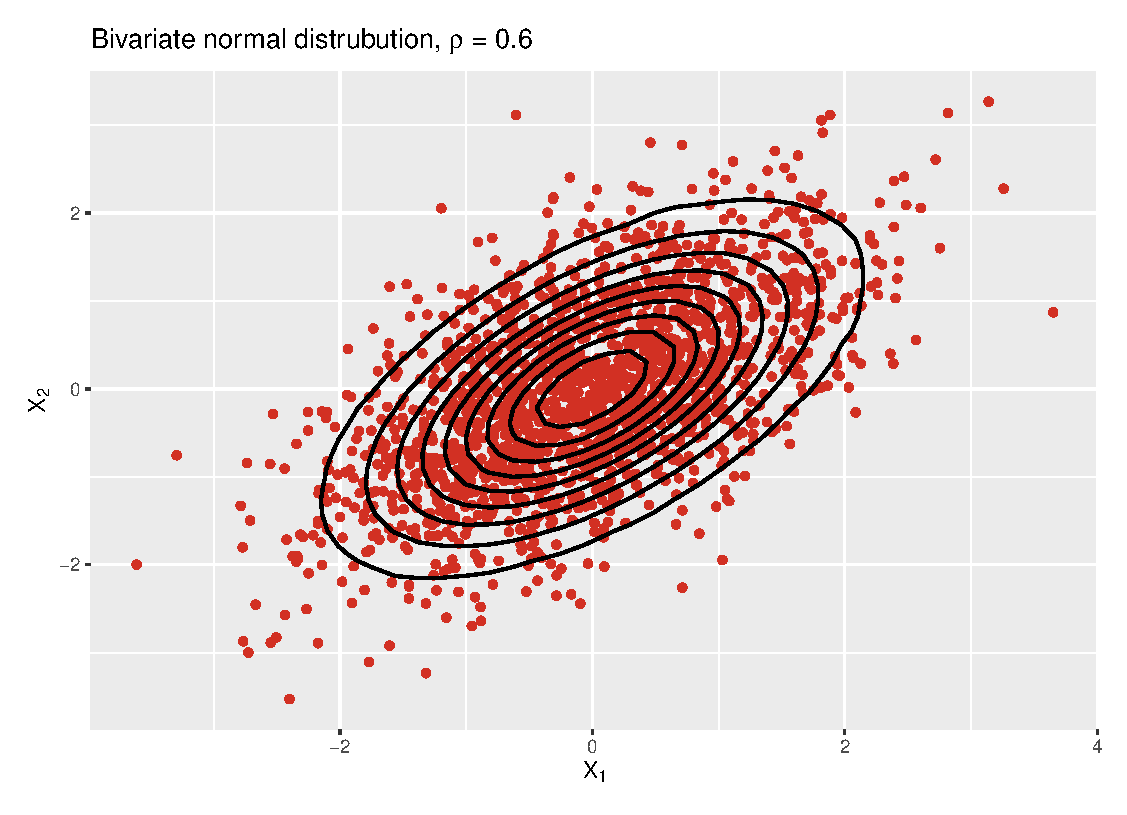
\includegraphics[width=\linewidth]{figures/bivariate_normal.eps}
  \caption{Gaussian distribution with contour lines}
  \label{fig:mvd_normal_copula}
\end{subfigure}
\begin{subfigure}{.45\textwidth}
  \centering
  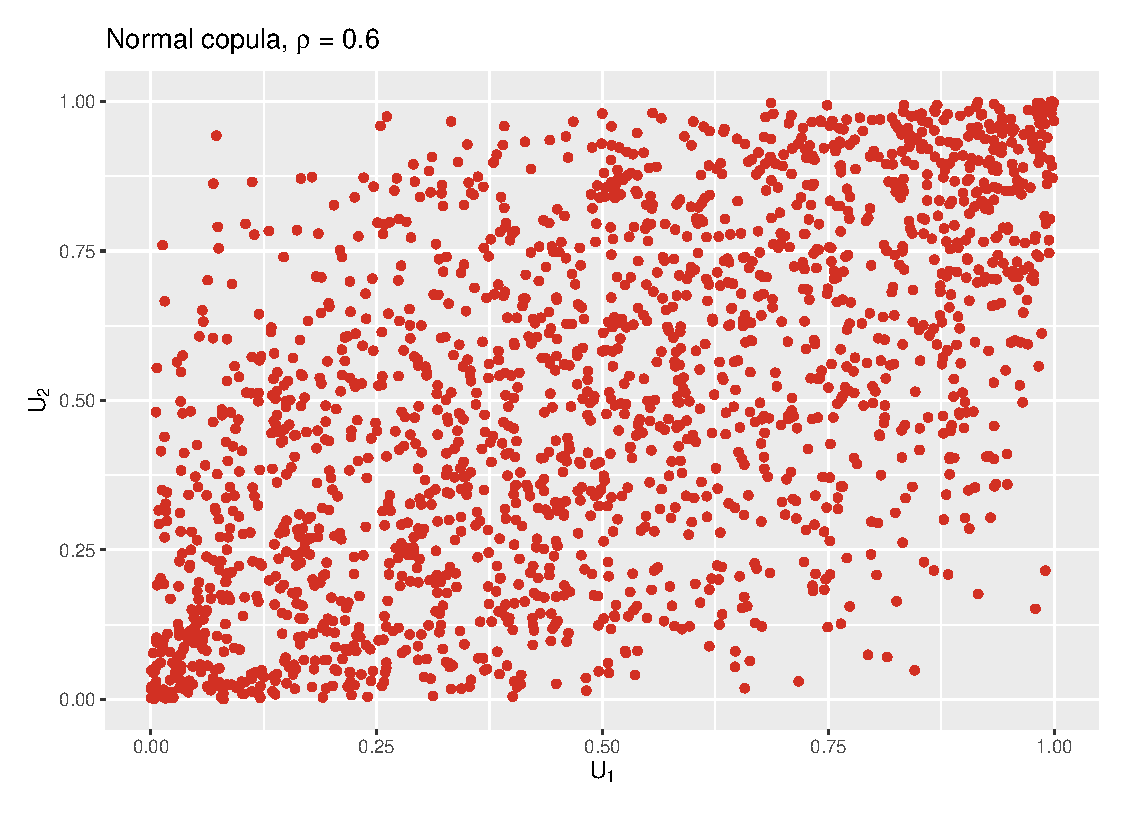
\includegraphics[width=\linewidth]{figures/normal_copula.eps}
  \caption{Gaussian copula}
  \label{fig:normal_copula}
\end{subfigure}
\caption{Bivariate Gaussian distribution and Gaussian copula for Pearson's $\rho = 0.6$ and simulated sample of size $n = 1800$, both with standard normal margins}
\label{fig:normal_plots}
\end{figure}






\textbf{t-Copula}\\
Consider without loss of generality $\bm{X} \sim {t_{d}(\nu, \bm{0}, \mathbf{P})}$ (multivariate Student's t-distribution) with $\nu$ \ac{dof} and $\bm{P}$ a correlation matrix, then the \textit{t-copula (family)} is given by
\begin{equation}
C_{\nu, \bm{P}}^{t}(\mathbf{u})=t_{\nu, \bm{P}}\left(t_{\nu}^{-1}\left(u_{1}\right), \ldots, t_{\nu}^{-1}\left(u_{d}\right)\right),
\end{equation}
where $t_{\nu}$ is the \ac{CDF} of the univariate Student's t-distribution  and $t_{\nu, \bm{P}}$ is the \ac{CDF} of the multivariate Student's t-distribution (both with $\nu$ \ac{dof}).\\
For the \textit{bivariate t-copula} ($d=2$), the special cases are the same as for the Gaussian copula, except that $d=0$ does not yield the independence copula (unless $\nu \rightarrow \infty$ in which case  $ C_{\nu, \rho}^{t} = C_{\rho}^{G a}$). The density of $C_{\nu, \bm{P}}^{t}$ is given by
\begin{equation}
c_{\nu, \mathbf{P}}^{t}(\boldsymbol{u})=\frac{\Gamma((\nu+d) / 2)}{\Gamma(\nu / 2) \sqrt{\operatorname{det} \mathbf{P}}}\left(\frac{\Gamma(\nu / 2)}{\Gamma((\nu+1) / 2)}\right)^{d} \frac{\left(1+\boldsymbol{x}^{\prime} \mathbf{P}^{-1} \boldsymbol{x} / \nu\right)^{-(\nu+d) / 2}}{\prod_{j=1}^{d}\left(1+x_{j}^{2} / \nu\right)^{-(\nu+1) / 2}},
\end{equation}
where $\bm{x} = \left(t_{\nu}^{-1}\left(u_{1}\right), \ldots, t_{\nu}^{-1}\left(u_{d}\right)\right)$.
\\

 \begin{figure}[H]
\centering
\begin{subfigure}{.45\textwidth}
  \centering
  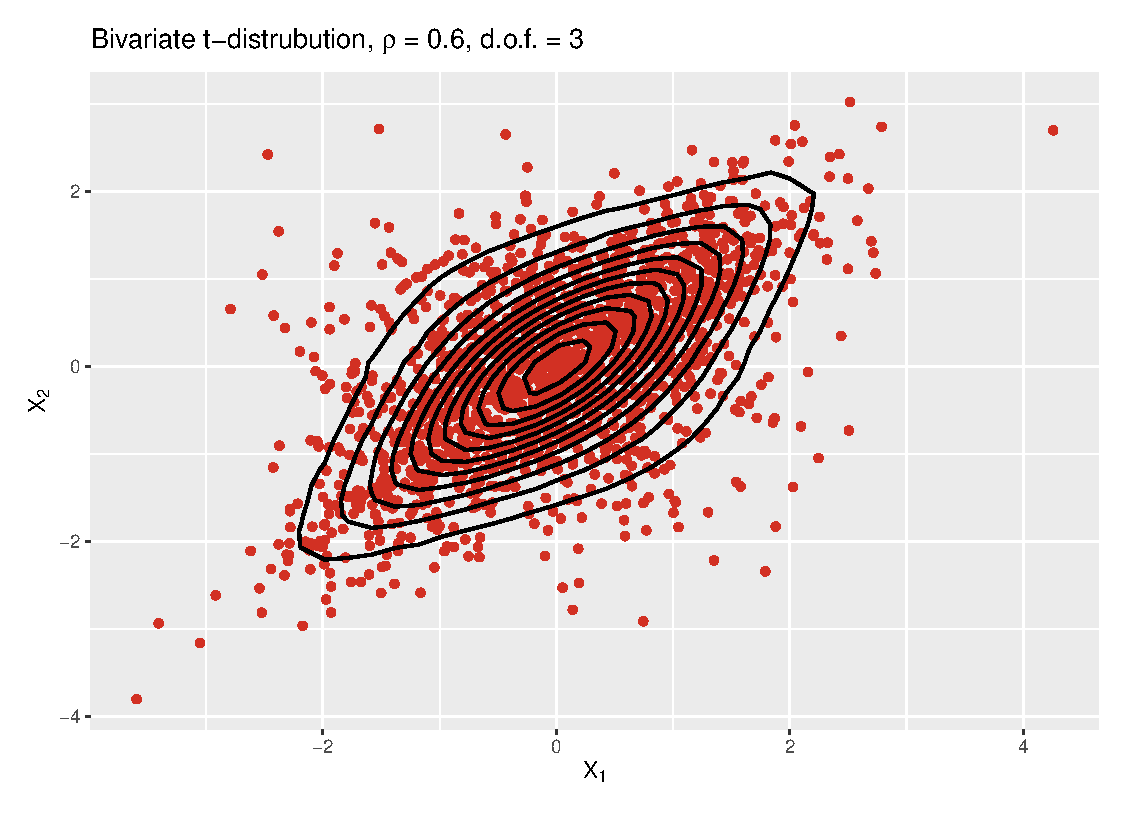
\includegraphics[width=\linewidth]{figures/bivariate_t.eps}
  \caption{t-distribution with contour lines}
  \label{fig:bivariate_t}
\end{subfigure}
\begin{subfigure}{.45\textwidth}
  \centering
  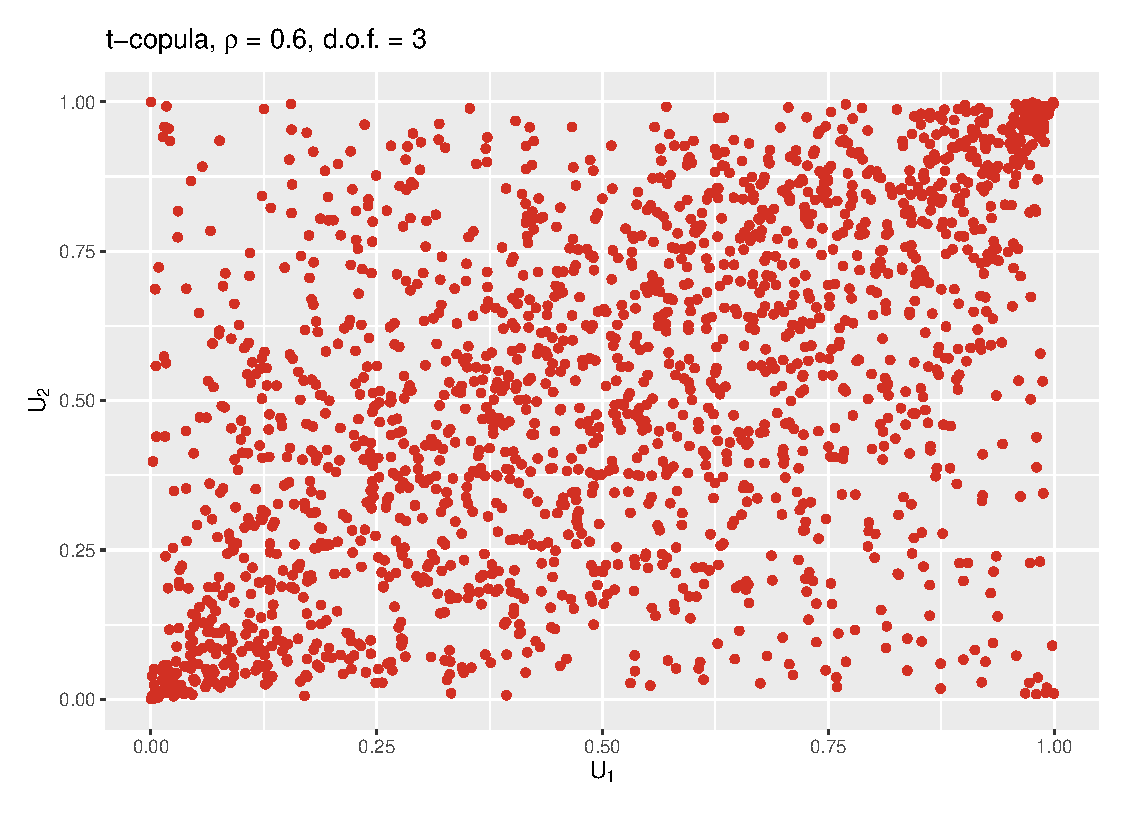
\includegraphics[width=\linewidth]{figures/t_copula.eps}
  \caption{t-copula}
  \label{fig:t_copula}
\end{subfigure}
\caption{Bivariate t-distribution and t-copula with 3 degrees of freedom for Pearson's $\rho = 0.6$ and simulated sample of size $n = 1800$, both with standard normal margins}
\label{fig:t_plots}
\end{figure}







\subsubsection{Archimedean Copulas} \label{sssec:archimedean_copulas}
% !TEX root = Master.tex

Unlike implicit copulas, \textit{explicit copulas} can be specified directly by taking into account certain constructional principles. The most important aspects of a such explicit copulas, in particular \textit{archimedean copulas}, are showcased in this subsection. Archimedian copulas are of the general form
\begin{equation}C(\boldsymbol{u})=\psi\left(\psi^{-1}\left(u_{1}\right)+\cdots+\psi^{-1}\left(u_{d}\right)\right),
\label{eq:archimedean_generator}
\end{equation}
where the function $\psi:[0, \infty) \rightarrow[0,1]$ is the \textit{(archimedean) generator} and satisfies the following properties:
\begin{itemize}
\item $\psi$ is strictly decreasing in the entire domain $[0, \infty)$
\item $\psi (0) = 1$
\item $\psi(\infty)=\lim \limits _{t \rightarrow \infty} \psi(t)=0$
\item We set $\psi^{-1}(0)=\inf \{t: \psi(t)=0\}$
\end{itemize}
If $\psi(t)>0, t \in[0, \infty)$, we call $\psi$ \textit{strict}. The set of all generators is denoted by $\Psi$.\\
Based on \autoref{eq:archimedean_generator} and the generator, we can construct several copula families. Three of the most popular ones are the \textit{Gumbel}, the \textit{Clayton} and the \textit{Frank} \textit{copula}.





\subsection{Dependence Measures} \label{ssec:dependence_measures}
% !TEX root = Master.tex

\textit{Dependence measures} allow us to summarize a particular kind of dependence into a single number in the bivariate case.
% Recall the Fr\'echet-Hoeffding bounds (\autoref{eq:frechet_hoeffding_lower} and \autoref{eq:frechet_hoeffding_upper}). They are an example of such kind of dependence measures. After all, they represent perfect negative or positive dependence.
In this section, we take a closer look into three classes of dependence measures along with appropriate association metrics.


\subsubsection{Linear Correlation} \label{sssec:linear_correlation}
% !TEX root = Master.tex

Undoubtedly, the most famous association metric for two \acp{RV} $X_1$ and $X_2$ is the \textit{Linear or Pearson's correlation coefficient}
\begin{equation}
\rho\left(X_{1}, X_{2}\right)=
\frac{\operatorname{Cov}\left(X_{1}, X_{2}\right)}{\sqrt{\operatorname{Var} (X_{1})} \sqrt{\operatorname{Var} (X_{2})}}
\in [-1, 1].
\label{eq:pearsons_rho}
\end{equation}
Note that $E(X_1) < \infty$ and $E(X_2) < \infty$ have to hold, i.e. the first two moments have to exist for $\rho$ to be defined.\\
The Pearson correlation coefficient is interpretable for \acp{RV} which have (approximately) a linear relationship, where $\rho = -1$ indicates perfect negative linear correlation, $\rho=1$ indicates perfect positive linear correlation and $\rho=0$ indicates no correlation between $X_1$ and $X_2$. However, comprehensibility of this measure comes along with some drawbacks:
\begin{itemize}
\item A correlation of $0$ is in general not equivalent to independence. This property holds only for normally distributed \acp{RV}.\footnote{e.g. $X_2 =X_1^2$ implies perfect dependence, yet $\rho(X_1,X_2) = 0$. Conversely though, independence always yields $\rho=0$.}
\item $\rho$ is invariant only under linear transformations, but not under transformations in general.
\item Given the margins and correlation $\rho$, one is able to construct a joint distribution only for the class of elliptical distributions. 
\item Given the margins, only for elliptically distributed \acp{RV} any $\rho \in [-1,1]$ is attainable.
\end{itemize}









\subsubsection{Rank Correlation} \label{sssec:rank_correlation}
% !TEX root = Master.tex

To compensate some of the drawbacks of linear correlation, we take advantage of correlation measures based on the ranks of data. \textit{Rank correlation coefficients}, like the ones presented below, are always defined and obey to the invariance principal. This means that these coefficients only depend on the underlying copula and they can thereof be directly derive.\\

\textbf{Spearman's Rho}\\
Consider two \acp{RV} $X_1$ and $X_2$ with continuous \acp{CDF} $F_1$ and $F_2$, then the \textit{Spearman's rho correlation coefficient} is simply the linear correlation between the \acp{CDF}
\begin{align}
\rho_{S}=\rho\left(F_{1}\left(X_{1}\right), F_{2}\left(X_{2}\right)\right).
\end{align}
The reason being is that by applying the \ac{CDF} to data, naturally a multiple of the ranks of the data are obtained, which essentially is equivalent to
\begin{equation}
\rho_S = \rho ( Ran(X_1), Ran(X_2) )
\end{equation}
Due to the invariance principle, we also obtain Spearman's rho directly from the unique copula via
\begin{equation}
\rho_{\mathrm{S}}=12 \int_{0}^{1} \int_{0}^{1} C\left(u_{1}, u_{2}\right) \mathrm{d} u_{1} \mathrm{d} u_{2}-3.
\end{equation}

\hfill $\square$ \\


\textbf{Kendall's Tau}\\
Let $X_1 \sim F_1$ and $X_2 \sim F_2$ be two \ac{RV} and let $(\tilde{X}_{1}, \tilde{X}_{2})$ be an independent copy\footnote{An independent copy $\tilde{X}$ of a RV $X$ is a RV that inherits from the same distribution as $X$ and is independent of $X$.} of $({X}_{1}, {X}_{2})$. Then \textit{Kendall's tau} is defined by 
\begin{equation}
\begin{aligned}
\rho_{\tau} &={E}\left[\operatorname{sign}\left(\left(X_{1}-X_{1}^{\prime}\right)\left(X_{2}-X_{2}^{\prime}\right)\right)\right] \\
&={P}\left(\left(X_{1}-X_{1}^{\prime}\right)\left(X_{2}-X_{2}^{\prime}\right)>0\right)-{P}\left(\left(X_{1}-X_{1}^{\prime}\right)\left(X_{2}-X_{2}^{\prime}\right)<0\right).
\end{aligned}
\end{equation}
Similarly to Spearman's rho, using the invariance principal, we can directly derive Kendall's tau from the unique copula by
\begin{equation}
\rho_{\tau}\left(X_{1}, X_{2}\right)=4 \int_{0}^{1} \int_{0}^{1} C\left(u_{1}, u_{2}\right) d C\left(u_{1}, u_{2}\right)-1.
\end{equation}

\hfill $\square$ \\


Both $\rho_S, \rho_{\tau} \in [-1,1]$, where any value within this interval is attainable in contrast to the Pearson coefficient. 
If any of these rank correlations is $-1$ (or $1$), we are in the countermonotonic (or comonotonic) case. If $\rho_S$ (or $\rho_{tau}$) $=0$, this does not necessarily imply independence between $X_1$ and $X_2$, although the opposite direction holds.
Furthermore, they are not limited to be invariant just under linear transformations . 











\subsubsection{Tail Dependence} \label{sssec:tail_dependence}
% !TEX root = Master.tex

\textit{Coefficients of tail dependence} express the strength of the dependence in the extremes of distributions, i.e. the joint tails. We distinguish between \textit{lower} and \textit{upper tail dependence} between $X_j \sim F_j, j = 1,2$ and provided that the below limits exist, they are given by
\begin{equation}
\lambda_{l}=\lim \limits _ {q \rightarrow 0^+} P \left(X_{2} \leq F_{2}^{\leftarrow}(q) | X_{1} \leq F_{1}^{\leftarrow}(q)\right) 
\label{eq:lower_tail_dependence}
\end{equation}
and 
\begin{equation}
\lambda_{u}=\lim \limits _ {q \rightarrow 1^-} P \left(X_{2} > F_{2}^{\leftarrow}(q) | X_{1} > F_{1}^{\leftarrow}(q)\right).
\label{eq:upper_tail_dependence}
\end{equation}
If $\lambda_l$ (or $\lambda_u$) $=0$, then we say that $X_1$ and $X_2$ are \textit{asymptotically independent} in the lower (or upper) tail,\footnote{Not necessarily true for the other way around} otherwise we have lower (or upper) tail dependence.\\
For continuous \acp{CDF} and by using Bayes' theorem, these expressions can be re-written to
$$
\begin{aligned}
\lambda_{l} &=\lim _{q \rightarrow 0^+} \frac{P\left(X_{2} \leq F_{2}^{\leftarrow}(q), X_{1} \leq F_{1}^{\leftarrow}(q)\right)}{P\left(X_{1} \leq F_{1}^{*}(q)\right)} \\
&=\lim _{q \rightarrow 0^+} \frac{C(q, q)}{q}
\end{aligned}
$$
and similarly
$$
\lambda_u = 2-\lim _{q \rightarrow 1^-} \frac{1-C(q, q)}{1-q}.
$$
Therefore, tail dependencies can be assessed by means of the copula itself when approaching the points $(0,0)$ and $(1,1)$. In addition, for all radially symmetric copulas (e.g. the bivariate Gaussian or the t-copula) we have $\lambda_l = \lambda_u = \lambda$.\\
Some examples are:
\begin{itemize}
\item Clayton: $\lambda_l = 2^{-1/ \theta}$, $\lambda_u = 0$ (only lower tail dependence)
\item Gumbel: $\lambda_l = 0$, $\lambda_u = 2 - 2^{1/ \theta}$ (only upper tail dependence)
\item Frank: $\lambda_l = 0$, $\lambda_u = 0$ (no tail dependence)
\end{itemize}
Following such guidelines, the choice of a practicable copula can be facilitated.





\subsection{Conditional Copulas} \label{ssec:conditional_copulas}
%% !TEX root = Master.tex

Modelling of the marginal response distributions along with their dependence structure has been studied so far in a strictly parametric context, not considering any potentially available covariate information. In this section, we will broaden the copula framework by adding conditions given possible covariates for all model parameters, i.e. both for the parameters of the marginals as well as the copula parameter. All involved model parameters will receive \textit{structured additive predictors} (see Section \ref{ssec:gam}) to account for possible non-linear or random effects. We will summarily explore \textit{Structured Additive Conditional Copulas} and for extensive literature, we refer to \cite{klein2016simultaneous} and \cite{vatter2019gamcopula}. \\

To get started, we define $(Y_1, Y_2)'$ to be independent bivariate responses\footnote{Continuous responses in the paper, but look at "A note on identification of bivariate copulas for discrete count data" to excuse this when explanatory variables are involved.} and $\bm{\nu}$ being the information contained in covariates. Ergo, \autoref{eq:sklar} of Sklar's theorem can be extended to the conditional case
\begin{equation}
F_{1,2}\left(Y_{1}, Y_{2} | \bm{\nu} \right)=C\left(F_{1}\left(Y_{1} | \bm{\nu} \right), F_{2}\left(Y_{2} | \bm{\nu} \right) | \bm{\nu} \right)
\label{eq:sklar_conditional}
\end{equation}
in conjunction with all facets of Section \ref{ssec:intro_to_copulas} \citep{patton2006modelling}.\\
The marginal \acp{CDF} $F_{d}\left(y_{i d} | \bm{\nu}_i\right)$ for observations $i = 1,\ldots, n$ can also be stated as
\begin{equation}
F_{d}\left(y_{i d} | \vartheta_{i 1}^{(d)}, \ldots, \vartheta_{i K_{d}}^{(d)}\right), \quad d = 1, 2,
\end{equation}
i.e. the distribution $F_d$ has a total of $K_d$ parameters, denoted as $\vartheta_{i 1}^{(d)}, \ldots, \vartheta_{i K_{d}}^{(d)}$.
To relate all parameters of the marginals to structured additive predictors $\eta_i^{\vartheta_k^{(d)}},  k = 1,\ldots, K_d$ consisting of the covariates $\bm{\nu}_i$ (see Section \ref{ssec:gam}), we employ strictly increasing response mappings $h_k^{(d)}$ to ensure proper domain allocation, i.e.
\begin{equation}
\vartheta_{i k}^{(d)}=h_{k}^{(d)}(\eta_{i}^{\vartheta_{k}^{(d)}}).
\label{eq:parameter_mapping}
\end{equation}
\\

Assuming that the parameters of the copula can also depend on covariates $\bm{\nu}_i$ while Sklar's theorem applies as usual, the left-hand side of \autoref{eq:sklar_conditional} can equivalently be stated as  
$$
F_{1,2}(y_{i 1}, y_{i 2} | v_{i})= F_{1,2}(y_{i 1}, y_{i 2} | \vartheta_{i 1}^{(1)}, \ldots, \vartheta_{i K_{1}}^{(1)}, \vartheta_{i 1}^{(2)}, \ldots,
\vartheta_{i K_{2}}^{(2)}, \vartheta_{i 1}^{(c)}, \ldots, \vartheta_{i K_{c}}^{(c)}),
$$
where the last share of parameters $\vartheta_{i 1}^{(c)}, \ldots, \vartheta_{i K_{c}}^{(c)}$ belong to the copula. Similar to \autoref{eq:parameter_mapping}, the copula parameters are modelled as $\vartheta_{i k}^{(c)}=h_{k}^{(c)}(\eta_{i}^{\vartheta_{k}^{(c)}})$ with $K_c$ being the number of parameters.














\subsection{Vine Copulas} \label{ssec:vine_copulas}
%% !TEX root = Master.tex

Vine copulas to be written down... 

\newpage
\thispagestyle{empty}
\cleardoublepage


\thispagestyle{plain}
\section{Data Exploration} \label{sec:data_exploration}
\newpage
\thispagestyle{empty}
\cleardoublepage

\thispagestyle{plain}
\section{Modelling} \label{sec:modelling}
\newpage
\thispagestyle{empty}
\cleardoublepage


\thispagestyle{plain}
\section{Conclusion} \label{sec:conclusion}
%% !TEX root = Master.tex

The objective of this study is to contribute to the development of LiDAR assisted forest inventories by developing
a statistical sound approach to derive unbiased diameter distribution models from LiDAR data for homogeneous
compartments of the forest. Prediction is successfully performed by a generalized linear
regression model using the gamma distribution with log as a link function. Clustering the compartments into three groups led to enough samples per cluster to
perform distribution engineering. Clustering is not meant to find groups upon a decision for more or less correction is made, but
to find an appropriate correction for similar compartments. Clustering further uncovered the issue of not detecting
equally height trees, which introduced additional bias in the tree diameter prediction. Bias correction is
achieved by fitting a gamma distribution on the diameter distribution of each cluster from the inventory dataset
and subsequently the predicted diameter distribution. A correction factor is calculated based on the ratio of the
shape and scale parameter of both fitted distributions for each cluster. High confidence is thus given to the
inventory dataset. Subsequently, the correction factor is applied for each section. \\

This approach could solve all present challenges, without relying on any heuristic methods apart from choosing
an appropriate amount of clusters and variables. Hence the objective of finding a statistical sound approach is achieved.\\

We could not find studies with similar approaches to the objective. 
The achieved residual standard error of the mean diameter of the corrected compartment distribution of 5.49cm (see Section \ref{Results}) is satisfying.
To compare and assess the modelling of the distribution, a inventory dataset of fully sampled compartments is necessary. 
The RSE could be further reduced by improving the tree species detection rate and likely crown area estimation. Comparing different amount of k cluster could be an interesting extension. 
The residual standard error of the regression model with 3.81cm is compared to another study. G. Liu, J. Wang, P. Dong, Y. Chen, Z. Liu (2018) [17] achieved a significantly better diameter residual standard error of 1.28 cm using solely LiDAR data. \textit{"Octree segmentation, connected component labelling and random Hough transform are comprehensively used to identify trunks and extract DBH of trees in sample plots."} \\

Nevertheless, this sophisticated approach can only be applied on plot level (small sampling location in a forest) and likely not scaled up on a whole forest. Ultimately, a residual standard error of below 5cm is satisfying. \\

The advantage of the presented approach is that an extension of the estimation of the unbiased tree diameter distribution based on just the LiDAR scanning system can be achieved, even though the majority of the area did not undergo any manual sampling activities.\\
Additionally, by making use of this bias correction attempt by fitting and adjusting parametric distributions instead of just relying on the predicted diameter distribution, outlier occurrences at the outer quantiles are no longer an issue (due to overestimated crown areas), meaning that overestimation of the tree diameter is also prevented. 




%\clearpage
\newpage
\thispagestyle{empty}
\cleardoublepage



\addcontentsline{toc}{section}{Appendix}
\thispagestyle{plain}
\section*{Appendix} \label{sec:appendix}
\input{appendix}
\newpage
\thispagestyle{empty}
\cleardoublepage



\addcontentsline{toc}{section}{List of Figures}
\thispagestyle{plain}
\listoffigures
\newpage
\thispagestyle{empty}
\cleardoublepage



\addcontentsline{toc}{section}{List of Tables}
\thispagestyle{plain}
\listoftables
\newpage
\thispagestyle{empty}
\cleardoublepage



\addcontentsline{toc}{section}{List of Abbreviations}
\thispagestyle{plain}
\section*{List of Abbreviations}
% !TEX root = Master.tex

\begin{acronym}
 
\acro{BIC}{Bayesian Information Criterion} 
\acro{GLM}{Generalized Linear Model}
\acro{LM}{Linear Regression Model}
\acro{LMM}{Linear Mixed Model}
\acro{GLMM}{Generalized Linear Mixed Model}
\acro{CDF}{Cumulative Distribution Function}
\acro{PDF}{Probability Density Function}
\acro{RV}{Random Variable}
\acro{wlog}[w.l.o.g.]{without loss of generality}
\acro{dof}[d.o.f.]{Degrees of Freedom}
\acro{GAM}{Generalized Additive Model}
\acro{GAMM}{Generalized Additive Mixed Model}
\acro{STAR}{Structured Additive Regression Model}
\acro{KC}{Key Category}
\acro{KCC}{Key Category Cluster}
%\acro{SB}{Sub-Brand}
%\acro{PD}{Product Division}
\acro{BS}{Business Segment}


\end{acronym}


\newpage
\thispagestyle{empty}
\cleardoublepage



\addcontentsline{toc}{section}{References}
\thispagestyle{plain}
% Insert bibliography and the bibliographic style
\bibliographystyle{dinat-en}
%Include references that are not explicitly cited in the documtent
\nocite{*} 
\bibliography{references}

\end{document}

